\documentclass[a4paper,11pt]{article}

\usepackage[utf8]{inputenc}

\usepackage{minted}

\usepackage{graphicx}

\begin{document}

\title{
    \textbf{How to sort an array: different ways}
}
\author{Ruxandra-Stefania Tudose}
\date{Fall 2023}

\maketitle

\section*{Introduction}

Since we have drawn the conclusion that operating on sorted data sets is much more efficient than working with unsorted 
ones, the question on the methods on how to actually sort the arrays inevitably arises. That is to say, this report aims 
to walk through the different sorting algorithms in order to analyze their complexity,
but at the same time to also identify the most efficient one.

\section*{An important remark}

In this experiment, an unsorted, randomly generated array has been used in order to then, be sorted. In order to compare and contrast 
different sorting approaches, it should be taken into consideration that the separate algorithms have been tested on the same cloned array.
Had it not been for the same data set, the conclusions related to the execution time or efficiency would have not been relevenat. 

\section*{Selection sort}

The goal of this algorithm is to go through the given array and to always look for the lowest element (if it exists) compared to the one currently 
pointing to. If found, the two interchange. This process keeps on going until the end of the array is reached. 
If we were to analyze the time complexity of the algorithm, we would have to look at the number of comparisons executed in an array of length n.
The first element will be compared to n-1 elements, the second one to n-2... and so on and so forth until the last one will be compared to itself.
Having said that, for the computation, the formula of the Gaussian sum has been used:

\[ \sum_{i=1}^{n-1} = \frac{(n-1)*(n-1+1)}{2} = \frac{n^2-n}{2}\] 

It can, therefore be concluded that \textit{the dominant term} in this expression is $n^2$. In other words, 
the selection sort's time complexity is \textbf{O($n^2$)}.
In order to get a better understanding of the description above, the code for the selection sort has been included: 


\begin{minted}{java}
public static void selsort (int [] array) {
    
    for (int i = 0; i < array.length; i++) {
   
       int candidate = i; //the index of the presumed possible min value
       for (int j = i; j < array.length ; j++) {
           if(array[j] < array[candidate]) {
               candidate = j;
           }
       }
       
        if(candidate != i)
            swap(array, i, candidate);
    }
}
\end{minted}
 
 

\section*{Insertion sort}

The goal of this algorithm is to always look back on the neighbour of the element pointing to (except for the first element in thre array).
If the two are disordered, they
will, therefore, swap. Unlike selection sort, one benefit of this algorithm is that it ensures that 
whatever is behind the element currently looking at is without
doubt, sorted. As previously mentioned, this process keeps on going until the end of the array is reached. \newline

If we were to analyze the time complexity of this algorithm, we would have to look at the number of comparisons executed in an array of length n.
Starting from the second element, it will be compared to one element only, the second one to two and so on and so forth until the last one will be compared to 
n-1 elements. Since it is the same formula as it is for the selection sort, the complexity of this algorithm will be \textbf{O($n^2$)} as well. \newline

\textit{Note:} This approach on the analysis of the time complexity only applies for the worst case scenario, which will be further 
explained in the next section.\newline\newline
Once again, in order to get a better understanding of the description above, the code for the selection sort has been included: 


\begin{minted}{java}

public static void insersort (int [] array) {

    for (int i = 0; i < array.length; i++) {
    //look back one position and check if the previous neighbours are disordered
        for (int j = i; j > 0 && array[j-1] > array[j] ; j--) { 
            swap(array, j-1, j); // if disordered - swap! 
        }
    }
}
\end{minted}

\subsection*{Interesting findings}

Even though at first, the swap operation may seem symmetrical, I was surprised that as far as the insertion sort is concerned, this is not necessarily the case.
And what do I mean by that is if first swapped \textit{j-1} with \textit{j} that will generate \textit{significantly} 
lower execution time than first swapping \textit{j} with
\textit{j-1}. \newline

The correct way of swapping in a for loop, in order to have faster execution times is as follows:

\begin{minted}{java} 
    
                    int tmp = array[j];
                    array[j]=array[j-1];
                    array[j-1] = tmp;

\end{minted}

After having run the benchmarks, I have come to the incredible conclusion that this apparently insignificant difference in which element is swapped first (as above)
is a bit over \textbf{2 times} faster. 
It should also be taken into consideration that in order to notice this difference, the swapping should be done inside the
for loop, not by calling a separately implemmented method!




\subsection*{Insertion vs. Selection sort: Which one is better so far?}

As far as the time complexity is concerned, what's interesting is that unlike the insertion sort, 
the selection sort algorithm does 
not have a best or worst case scenario. That is to say, regardless of the array, the number of the comparisons will be the same. 
I will always have to go through the set of data from the 
beginning until the end in order to look for a potential minimum value. In other words, this is among others, a reason why this algorithms is not efficient.

On the other hand, in terms of the number of swap operations that have to be executed, those will depend on the initial array for both algorithms.\newline   

\begin{table}[h!]
    \centering
    \begin{tabular}{||c c c c c||} 
    \hline
    Type & TimeCBest & TimeCWorst & SwapBest & SwapWorst\\ [0.5ex]
    \hline
    SelectionSort& O($n^2)$ & O($n^2)$ & 0 & O(n)\\
    InsertionSort & O(n) & O($n^2)$ &  0 & O($n^2)$ \\ [1ex] 
    \hline
    \end{tabular}
    \caption{Complexity analysis of the insertion and selection sort.} 
    \label{table:1}
\end{table}

The question that now arises is, as far as the resources are concerned, which out of the options we have is more expensive. The choice is therefore,
between an inefficient swap operation (for the insertion sort, in its worst case) 
or  always going through an array regardless of the case we find ourselves in and keeping on comparing the values 
(that is because selection sort is \textit{O($n^2$)} all the time).
All in all, in terms of time and resources reading and writing costs more than swapping. During those two operations, stalling may occur because of 
register conflicts or simply because the whole process has to temporarily stop since there is one missing value that is to be calculated.\newline\newline
In other words, in our analysis so far, \textit{insertion sort} is the most efficient, being approximately \textbf{3 times} faster than selection sort.

\section*{Merge sort}

The approach of the merge sort algorithm is completely different compared to the ones presented until now. Not only is it used recursively,
but it also takes advanted of executing unrelated operations on separate cores simultaneously, which of course saves time during execution.
The goal is to always split the array into two separate smaller arrays, to sort them and then to merge them back into one array. This process is done
recursively until an array of one element only is reached (we reach \textit{n levels}). That is precisely why its complexity is \textit{$n*logn$}\newline
Since we have already come to the conclusion that insertion sort is more efficient than selection sort, 
it will be the one used to analyze how it performs in comparison with merge sort.\newline

\begin{table}[h!]
    \centering
    \begin{tabular}{||c c||} 
    \hline
    ArraySize & Ratio \\
    \hline
    1000 & 3.3 \\
    2000 & 17.8 \\ 
    4000 & 5.2 \\ 
    8000 & 12.6 \\ 
    16000 & 23.6 \\ [0.5ex]
    \hline
    \hline
    \end{tabular}
    \caption{The ratio between insertion and merge sort.} 
    \label{table:2}
\end{table}

\textit{Note: } For the above analysis the fast version of the insertion sort has been taken into
consideration in order to calculate the ratio.

\begin{figure}[ht]
    \centering
    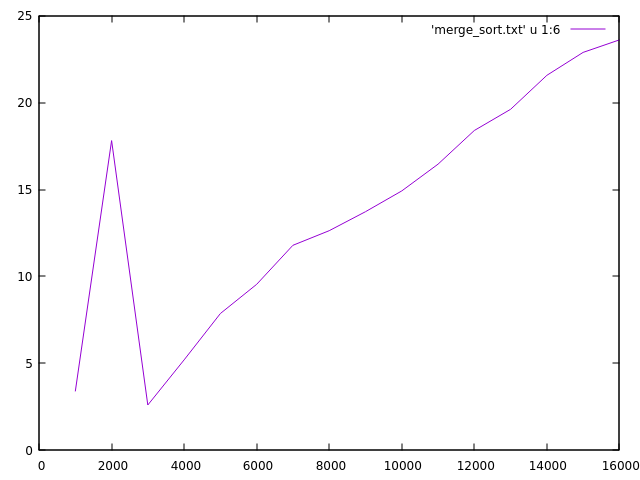
\includegraphics[width=0.8\textwidth]{merge_sorted_ratio.png}
    \caption{The graph describing the evolution of the ratio between insertion and merge sort.}
    \label{fig:1}
\end{figure}

Although there is a spike (where the x-axis is 2000), namely an isolated case, that should not affect our conclusions
simply because the arrays are randomly generated and it's high chances at some point we may get a favourable case for one of the algorithms. 
The rest of the values indicate a step by step increase in the ratio's value, namely the larger the data set, the more efficent merge sort becomes and 
on average according to my experiment, it is \textbf{13 times} faster.

\subsection*{An even better version of merge sort}

It seems that merge sort can undoubtedly be optimised, namely by avoiding all the copying in the merge operation since it takes
up a lot of time and resources to do so. And we can do so by first, cloning the initial array and then, in the recursive step by simply toggling the array arguments.
After having run my benchmark, I have obtained that this improvement is approximately \textbf{3 times} faster than the initial version of the merge sort. \newline\newline
What's more is that even though at first, the ratio between the two algorithms varies unpredictably,
it seems that it stabilizes as the arrays increase (after the x-axis takes value 10000), as it can be seen below: \newline\newline

\begin{figure}[ht]
    \centering
    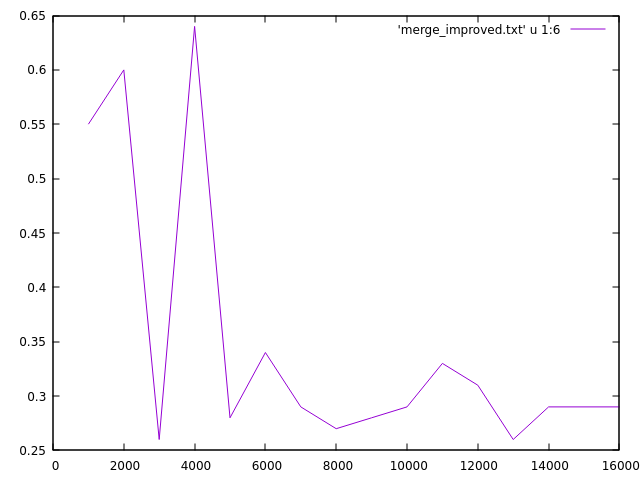
\includegraphics[width=0.8\textwidth]{merge_improved.png}
    \caption{The graph describing the evolution of the ratio between the older and improved version of merge sort.}
    \label{fig:1}
\end{figure}


\section*{Conclusion}

All in all, there are several ways of sorting an array, however after having run this experiment, turns out merge sort is the most efficient algorithm not only
by looking at its time complexity and in it executing unrelated operations on different cores, but also because of its ability
in being improved by avoiding most of the
copying, as stated above.


\end{document}